\chapter{Einleitung}

\noindent Generative Adversarial Networks (GANs) haben in den letzten Jahren erhebliche Aufmerksamkeit in der Forschungsgemeinschaft auf sich gezogen. Sie stellen eine neue Methode dar, um generative Modelle zu trainieren und haben eine Vielzahl von Anwendungen in Bereichen wie Bildsynthese, Super-Resolution und Style Transfer. \\

\noindent Das Ziel dieser Arbeit ist es, einen umfassenden Überblick über GANs zu geben, ihre Funktionsweise zu erklären und einige der Herausforderungen zu diskutieren, die bei ihrer Implementierung und ihrem Training auftreten. \\

\begin{wrapfigure}{l}{0.50\textwidth}
    \centering
    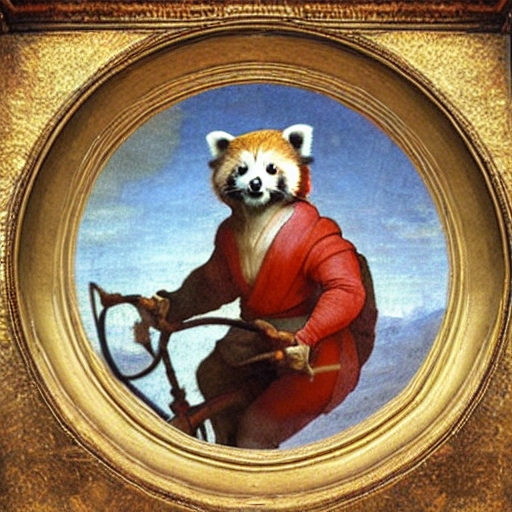
\includegraphics[width=0.50\textwidth]{red-panda-riding-a-unicycle}
    \caption{Beispiel für ein Bild, das von einem GAN generiert wurde. Ausgangssatz: „Ein roter Panda, der ein Einrad fährt“}
    \label{Abb:basic}
    \end{wrapfigure}

\hfill
\break
Das Paper ist wie folgt strukturiert: Nach dieser Einleitung werden in Kapitel 2 die Grundlagen von neuronalen Netzen, Deep Learning und generativen Modellen erläutert. Kapitel 3 ist den GANs gewidmet, wobei ihr Konzept, ihre Architektur und ihr Training im Detail besprochen werden. Kapitel 4 behandelt verschiedene Anwendungen von GANs, während Kapitel 5 einige der Herausforderungen und Lösungsansätze bei der Arbeit mit GANs diskutiert. Schließlich werden in Kapitel 6 Schlussfolgerungen gezogen und ein Ausblick auf zukünftige Forschungsrichtungen gegeben. \\